%
% This is the Appendix A file (appA.tex)
%
\appendix{Flux functions and initial condition}
\label{sec:flux}

We define the influx and outflux functions $Q_{lg}$, $Q_{p}$ to be bump functions in space and time. With
\begin{equation}
\step(x,a,b) = 1/2 (1 + \tanh[(4 (a + b - 2 x))/(a - b)]),
\end{equation}
we define a indicator like bump function
\begin{equation}
w(x,a,b,l) = \step(x,a,a+l)-\step(x,b-l,b)
\label{indicator_fun}
\end{equation}
that has support on $[a,b]$ but continuously drops from 1 to 0 in intervals of length $l$. Here $w$ effectively is a smooth approximation of an indicator function. 

 With this bump function and a blink cycle with period $L$, we define
\begin{eqnarray}
\hat{Q_{lg}}(\hat{x},t) &= w(t,0.02,0.5 L,0.1) \exp(((\hat{x}-0.5)/0.25)^2), \label{bumb_funs}  \\
\hat{Q_{p}}(\hat{y},t) &= w(t,0.05,0.5 L,0.1) w(\hat{y},-0.9,0.25,0.9). 
\end{eqnarray}
With target supply and drain volumes $V_s, V_d$ over a blink cycle, we normalize the flux functions (\ref{un_flux}) to define $Q_p,Q_{\lg}$:
\begin{eqnarray}
Q_{lg}(\hat{x},t) &= \frac{V_s}{\int_{0}^{p} \int_{-1}^1 \hat{Q_{lg}} d\hat{x} dt} \hat{Q_{lg}}(\hat{x},t), \label{un_flux1} \\
Q_{p}(\hat{y},t) &= \frac{V_d}{\int_{0}^{p} \int_{-1}^1 \hat{Q_{p}} d\hat{y} dt} \hat{Q_{p}}(\hat{y},t).
\label{un_flux}
\end{eqnarray}
The influx function $Q_{lg}$ is defined so there is an influx of fluid from the top of the lid, concentrated in the towards the right; this is simulated with the use of an exponential bump function, as seen in (\ref{un_flux1}). The influx occurs for $t \in [0.02,0.5 L]$. The ouflux function $Q_p$ defines a drainage through the puncta; $Q_p$ is defined on the left corner of the eye-shaped domain. The outflux occurs evenly throughout the corner, as seen with the use of the indicator like function (\ref{indicator_fun})  in (\ref{un_flux}). The outflux occurs within $t \in [0.05,0.5 L]$, starting after an initial influx of fluid. A plot of the flux functions at different times throughout the blink cycle can be seen in Figure~\ref{flux_plots}.

\begin{figure}
	\centering
	\subfloat[]{
		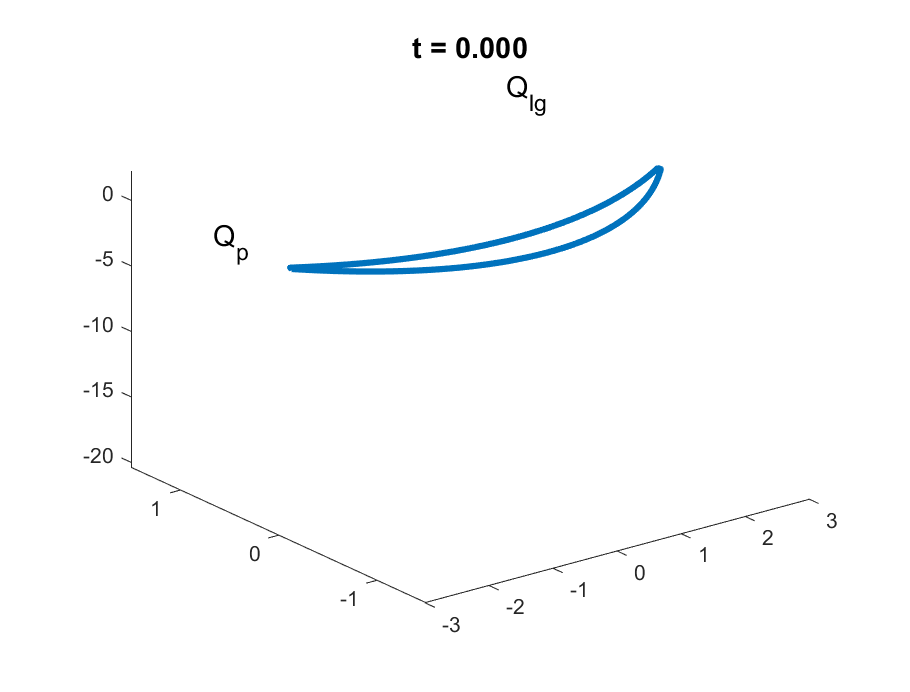
\includegraphics[scale = 0.4]{Chapter4/fluxfuns1}
		\label{flux_plot1}
	}
	\subfloat[]{
		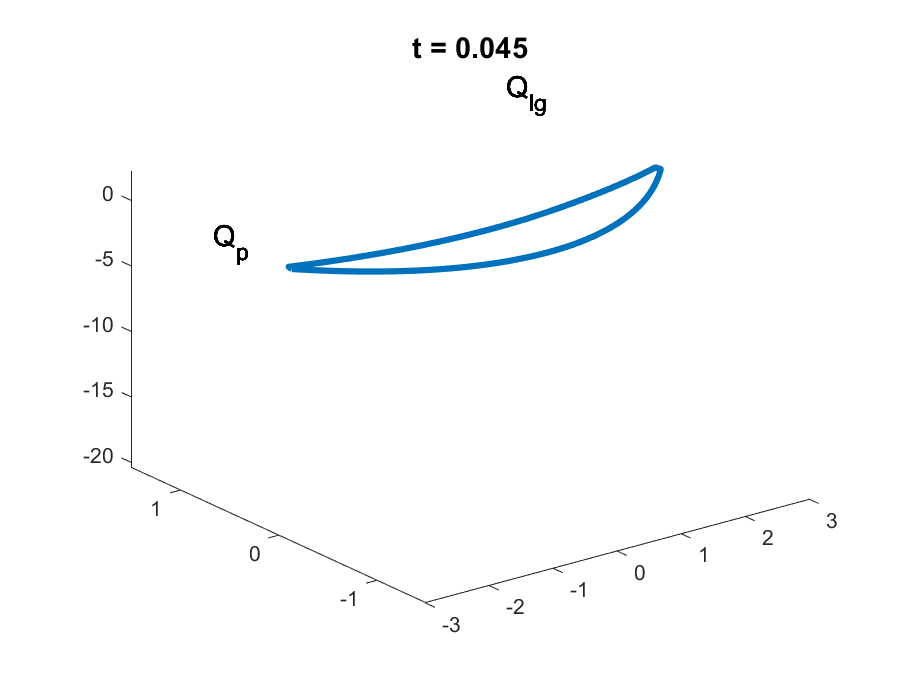
\includegraphics[scale = 0.4]{Chapter4/fluxfuns2}
		\label{flux_plot2}
	} 
	
	\subfloat[]{
		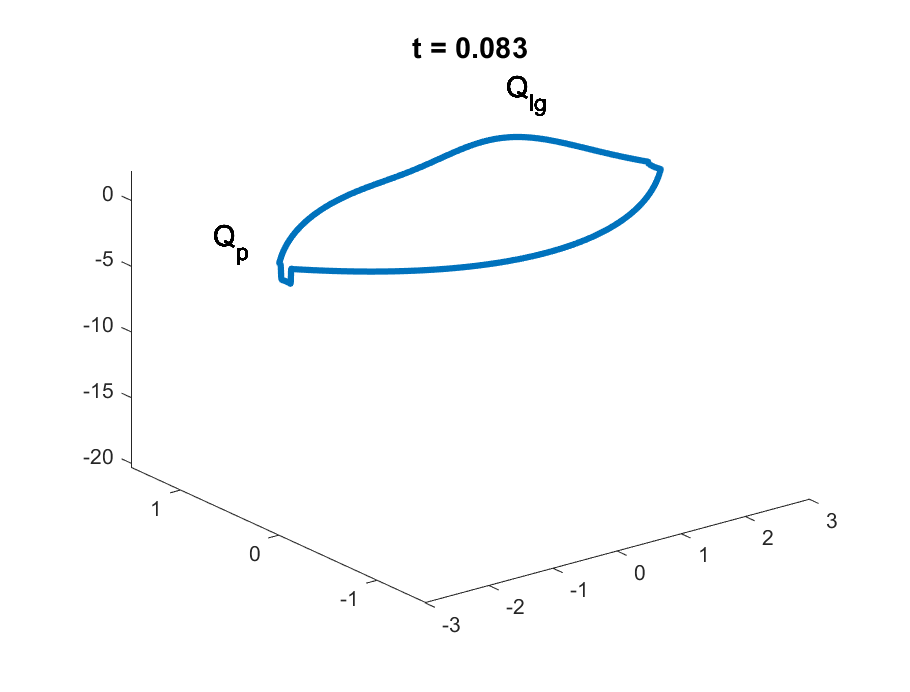
\includegraphics[scale = 0.4]{Chapter4/fluxfuns3}
		\label{flux_plot3}
	}
	\subfloat[]{
		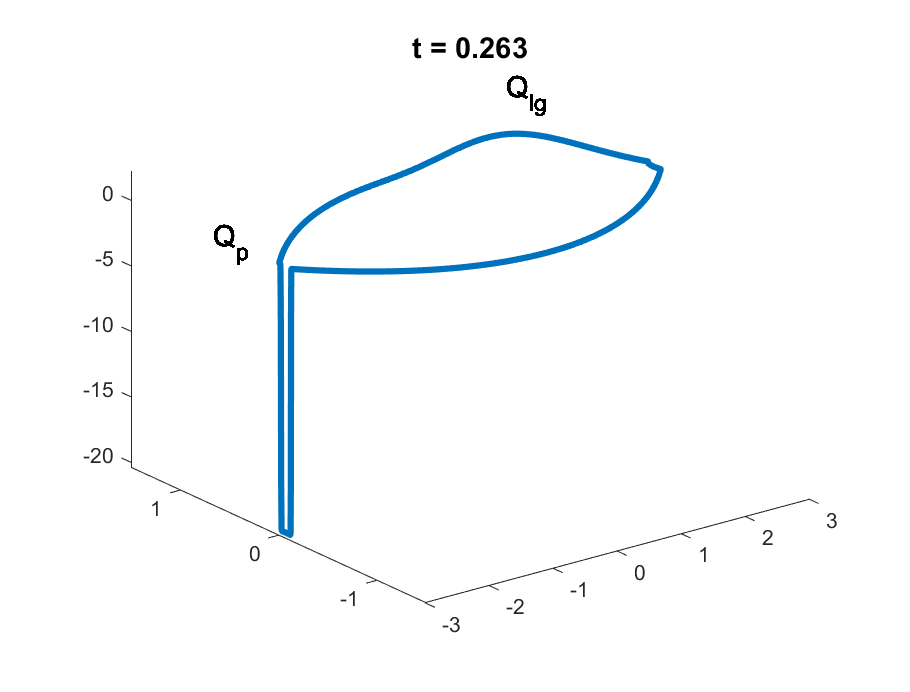
\includegraphics[scale = 0.4]{Chapter4/fluxfuns4}
		\label{flux_plot4}
	} 
	
	\subfloat[]{
		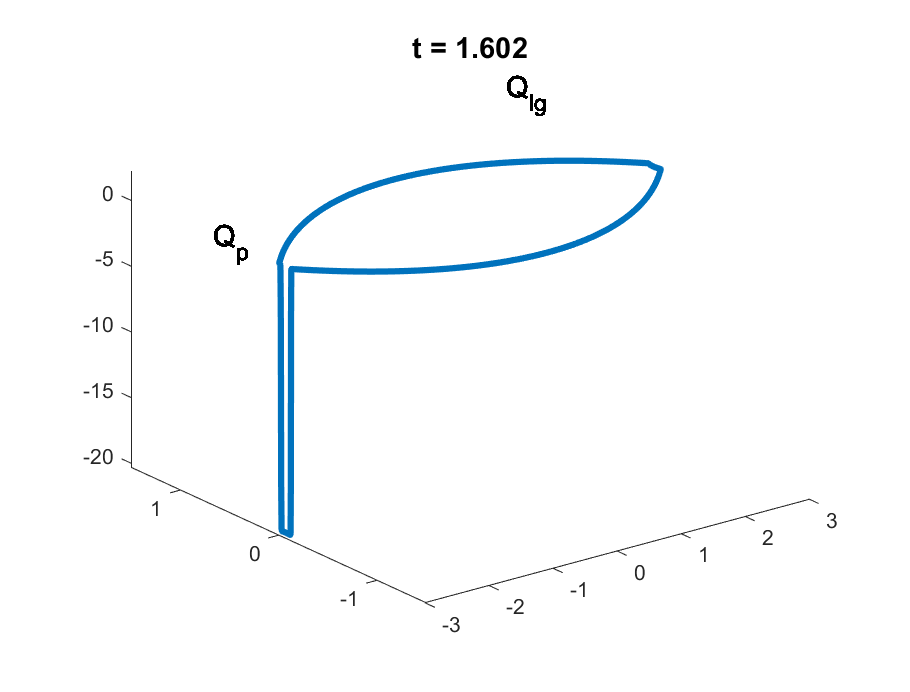
\includegraphics[scale = 0.4]{Chapter4/fluxfuns5}
		\label{flux_plot5}
	}
	\subfloat[]{
		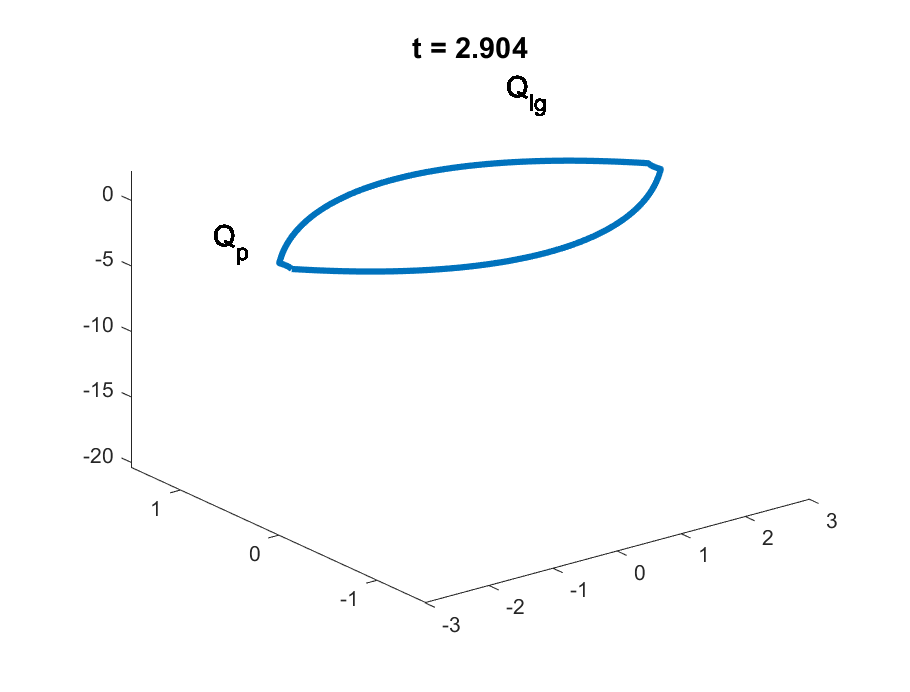
\includegraphics[scale = 0.4]{Chapter4/fluxfuns6}
		\label{flux_plot6}
	}
	
	\caption{Plot of the flux functions (\ref{un_flux1},\ref{un_flux}) at different times throughout the blink cycle. At the start of the blink cycle both fluxes are 0. Then at $t=0.02$, an influx of fluid starts, followed by an outflux at $t=0.05$. From $t=0.05$ to $t=0.5 L$, there is both an influx and outflux of fluid. After $t=0.5 L$, both the influx and outflux of fluid dissipates.}
	\label{flux_plots}
\end{figure}

We define the initial condition $h_I(\hat{x},\hat{y})$ implicitly by first solving
\begin{align}
\begin{aligned}
\nabla^2 \hat{h_I} &= 10 (\hat{x}^4 +\hat{y}^4) \quad (\hat{x},\hat{y}) \in \mathcal{C} \\
\hat{h_I} &= 1 \mbox{ on } \partial \mathcal{C},
\end{aligned} 
\end{align}
and finding coefficients $c_0,c_1$ so that the initial condition
\begin{equation}
h_I(\hat{x},\hat{y}) = c_1 \hat{h_I}(\hat{x},\hat{y})+c_0
\end{equation}
matches $h_0$ on the boundary and numerically has a prescribed volume $V_{\mbox{init}}$. This initial condition produces a solution with boundary layers, as seen in Figures~\ref{tears_02_1},\ref{broken_tears_0}.